\subsubsection{Elliptic curves over finite fields}
Now that the groundwork for elliptic curves has been laid, we are ready to address the main subject matter, that of elliptic curves over finite fields.
As stressed before, we restrict our attention to finite fields $\fp$ of the form $\zn[p]$, the integers modulo a prime $p$.
% Weierstrass or normal form?
We also take all curves to be in Weierstrass form from here out, and only look at the affine parts of the curves.
The underlying field $k$ of $\an$ and $\pn$ we now take to be $\fp$ instead of $\C$ for the rest of the document, unless otherwise specified.
% FF<-0:28
% 
% # curve is y^2 = 4x^3 + 2x + 1
% 
% xpoints<-numeric()
% ypoints<-numeric()
% 
% for(x  in FF){
%   for(y in FF){
%     if((y^2)%%29==(4*x^3 + 2*x +1)%%29){
%       xpoints<-c(xpoints,x)
%       ypoints<-c(ypoints,y)
%     }
%   }
% }
% 
% plot(xpoints,ypoints,xlab="x",ylab="y")
% 
Therefore we still write curves as $E:y^2=f(x)$, except now, by changing the field $k$, we have coefficients of $f(x)$ and points on the curve $(x,y)$ with values in $\fp$, and so the visible part of an elliptic curve $E$ is represented by a collection of points in $\an[2](\fp)$.
The point at infinity $\pai$ remains on the curve at $[0,1,0]$.
\Cref{finitecurve} gives a visual example of a curve over a finite field.
\begin{figure}[htbp]
	\centering
	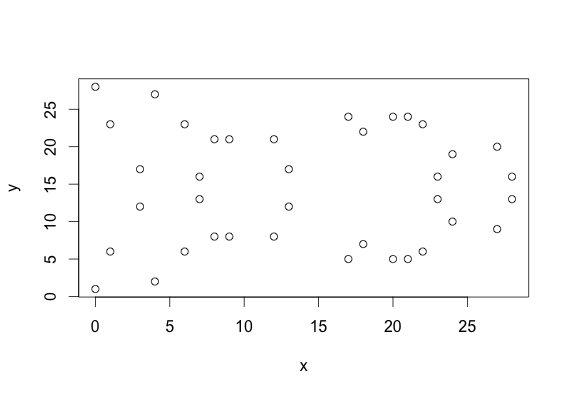
\includegraphics[scale=0.5]{../Figures/finiteellipticcurve.png}
	\caption{The curve $y^2 = 4x^3 + 2x + 1$ over $\fp[29]$}
	\label{finitecurve}
\end{figure}
\subsubsection{Addition formulae for points}
For elliptic curves over a finite field $\mathbb{F}_p$, when adding points $(x_1,y_1) + (x_2,y_2) = (x',y')$,
$$x'=\lambda^2 - a - x_1 - x_2,\quad y' = \lambda x_1 -\lambda x' - y_1 $$
where $\lambda = \frac{y_2-y_1}{x_2-x_1}$ if $x_1\neq x_2$ or $\lambda=\frac{3x_1^2 + 2ax_1 + b}{2y_1}$ otherwise.
These formulae are only valid when neither $(x_1,y_1)$ nor $(x_2,y_2) = \pai$, since $\pai$ has no coordinates in $\fp \times \fp$.

It is important to remember that we are now dealing with arithmetic in $\fp$, and so the division referenced is actually multiplication by the inverse element in $\fp$, which can be found with the euclidean algorithm as before.
Another consequence is that all calculations are performed $\mod p$.
